\clearpage
\Question{Tries}

Consider the following ternary search trie (TST):
\begin{center}
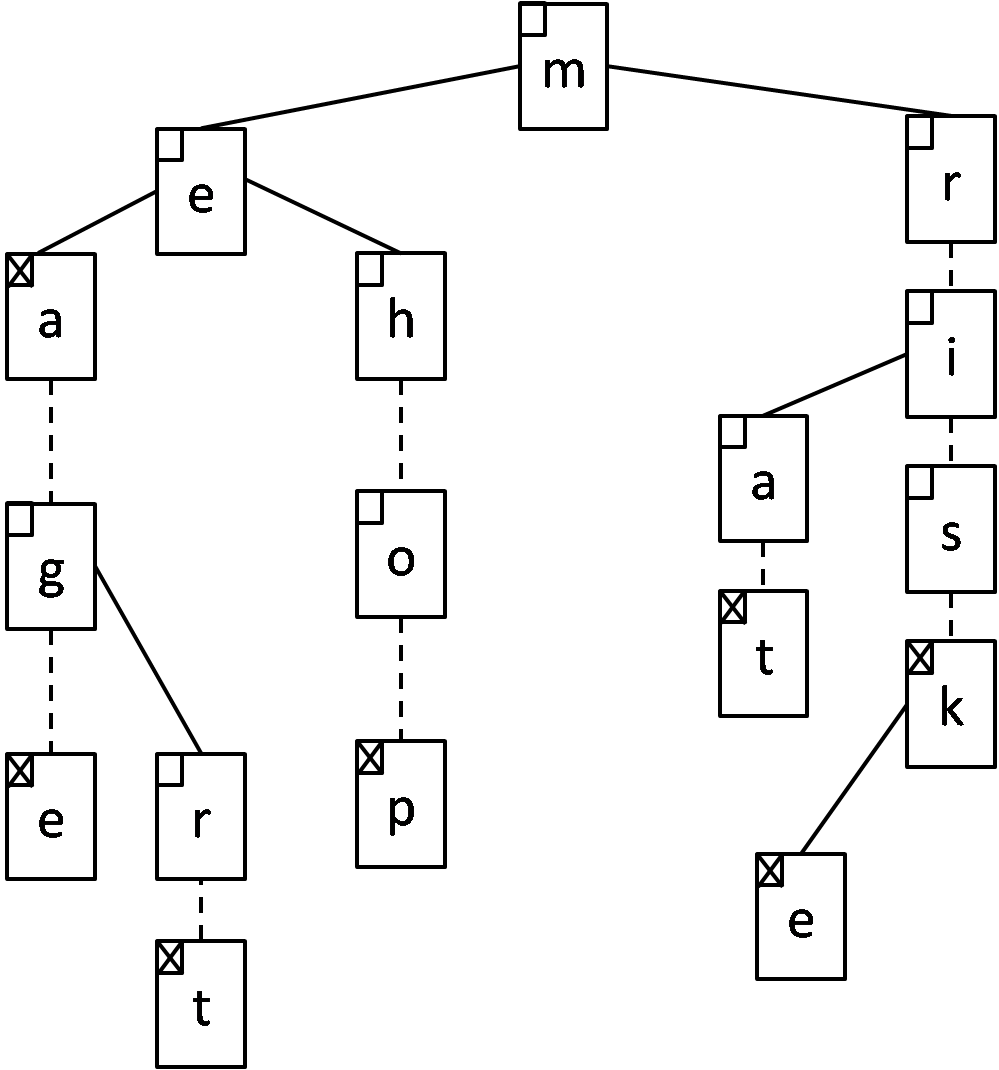
\includegraphics[width=.6\textwidth]{\img/tst2.png}
\end{center}

The dotted lines connect a node to its middle child, and solid lines
connect a node to its left and right children.  An \emph{X} in the top
left indicates that this node ends a valid word.


A desirable invariant of TSTs is that if the middle child is
\lstinline'NULL', the node has to end a valid word. This TST does not have
this invariant due to the topmost \lstinline'm' and \lstinline'e' nodes, but it
is not a necessary invariant for safety or correctness. (The insertion
and lookup algorithms work even without that invariant.)

\begin{parts}

\part[2]\TAGS{trie}
List all of the valid words stored in the TST above, in alphabetical order.
\begin{framed}
\ifprintanswers{\color{\answerColor}
  A, AGE, ART, HOP, RAT, RISK, RISE
}\else~\vspace{1.0in}\fi
\end{framed}

\RUBRIC
Part (a)
TAGS: trie

Gradescope rubric:  TODO

Commentary:
  A, AGE, ART, HOP, RAT, RISK, RISE
  Half a point penalty if not alphabetical order
  Half point penalty for each missing/incorrect word
  Minimum of 0
ENDRUBRIC

\newpage
\part[1]\TAGS{trie}
Add the words
\lstinline'me',
\lstinline'rake',
\lstinline'hope',
\lstinline'hot',
\lstinline'top', and
\lstinline'act'
to the TST given on the previous page, one at a time, in the order
given.  DO not worry about rebalancing
\begin{framed}
\begin{lstlisting}[basicstyle=\basicstyle\color{\answerColor}]
           ----------m*-------
          /          |        \
     ----e--         E*        r--
    /       \                  |  \
   a*        h             ----i   T
   |         |            /    |   |
  -g--       o           a     s   O
 / |  \      |           |     |   |
C  e*  r     p--         t*  --k*  P*
|      |     |  \           /
T*     t*    E*  T*         e*
\end{lstlisting}
\else~\vspace{8.0in}\fi

\RUBRIC
Part (b)
TAGS: trie

Gradescope rubric:  TODO

Commentary:
  - Half point per missed or incorrect insertion until they hit 0
      - CT to the left of "e"
      - E below "hop"
      - T to the right of "hop"
      - E below "m"
      - TOP to the right of "r"
  - Max 2 half-point penalties for screwed up Xes

(original TST in lowercase, additions in uppercase)
           ----------m*-------
          /          |        \
     ----e--         E*        r--
    /       \                  |  \
   a*        h             ----i   T
   |         |            /    |   |
  -g--       o           a     s   O
 / |  \      |           |     |   |
C  e*  r     p--         t*  --k*  P*
|      |     |  \           /
T*     t*    E*  T*         e*
ENDRUBRIC

\newpage
\part[3]\TAGS{correctness, loop-invariant, trie}
For this question, review the published code for tries from lecture.

It is possible to implement \lstinline|trie_lookup| as an iterative
function rather than a recursive one. Fill in the blanks so that the
function shown below correctly implements lookup in a TST.

The lines involving the variables \lstinline|lower| and
\lstinline|upper| are used only to prove that the loop invariant
(written in the incorrect location as an assertion in the code below)
is preserved. You should not use \lstinline|lower| or
\lstinline|upper| when filling in the blanks.
\begin{framed}
\begin{lstlisting}
elem trie_lookup(trie TR, char *s) {
    REQUIRES(is_trie(TR));
    REQUIRES(s != NULL);
    tnode *T = TR->root;
    int charmin = 0;
    int charmax = (int)CHAR_MAX + 1;
    int lower = charmin;
    int upper = charmax;

    while (T != [*\uanswer{27.5em}{NULL}*]) {
       ASSERT(is_tnode(T, lower, upper)); // Loop invariant
       if (*s == T->c) {
           if (*(s+1) == '\0') {

               return [*\uanswer{25.5em}{T->data}*];
           } else {
               lower = charmin;
               upper = charmax;
               s++;

               T = [*\uanswer{27em}{T->middle}*];

       } else if ([*\uanswer{26.5em}{*s > T->c}*]) {
           lower = T->c;

           T = [*\uanswer{29em}{T->right}*];

       } else {
           upper = T->c;

           T = [*\uanswer{29em}{T->left}*];
       }
    }
    return NULL;
}
\end{lstlisting}
\end{framed}

\RUBRIC
Part (c)
TAGS: correctness, loop-invariant, trie

Gradescope rubric:  TODO

Commentary:
  +0.5 per blank

Solution:
elem trie_lookup(trie TR, char* s) {
  REQUIRES(is_trie(TR));
  REQUIRES(s != NULL);
  tnode* T = TR->root;
  int charmin = 0;
  int charmax = (int)CHAR_MAX + 1;
  int lower = charmin;
  int upper = charmax;

  while (T != NULL) {
    ASSERT(is_tnode(T, lower, upper)); // Loop invariant
    if (*s == T->c) {
      if (*(s+1) == '\0') {
        return T->data;
      } else {
        lower = charmin;
        upper = charmax;
        s++;
        T = T->middle;
      }
    } else if (*s > T->c) {
      lower = T->c;
      T = T->right;
    } else {
      upper = T->c;
      T = T->left;
    }
  }
  return NULL;
}
ENDRUBRIC


\end{parts}
